% =============================================================
% STRATA — short paper (12 pages of body + references + appendix)
% Condensed from paper/paper-v2.tex (the long manuscript, 2026-09-28).
% Bibliography: ../references.bib   Figures: ../figures/
% UREAP 2026, Thompson Rivers University
% Author: Yassh Singh
% Supervisors: Dr. Anthony Aighobahi, Dr. Mridula Sharma
%
% RULE OBSERVED IN THIS FILE: every number appears in paper-v2.tex or in a
% committed artefact under outputs/ (x33_coverage_*.json, x38_guideline36.json,
% alarm_attribution.json, component_attribution.json, x37_diagnosis.json,
% x35_field_conditions.json, x36_quantile_band.json, x26_real_data_budget.json,
% intervals.json, crywolf.json, union_fpr_*.json, benchmark_v6_*.json).
% Framing (author's rule): lead with what the framework achieves; limitations
% are limitations, stated after. Process mining helps to get detection but it
% is not detecting on its own: the stratified structure (unit/device strata,
% event abstraction from the control sequence, absence and frequency channels)
% carries localisation and detections; conformance checking of discovered nets
% alone does not detect, and that is a finding. No number changed, no fired
% falsifier removed.
% Review loop: docs/reviews/2026-09-28-short-paper-review-loop.md
% =============================================================

\documentclass[11pt,letterpaper]{article}

\usepackage[margin=1in]{geometry}
\usepackage{microtype}
\usepackage[hidelinks]{hyperref}
\usepackage{cite}
\usepackage{times}
\usepackage{graphicx}
\usepackage{array}
\usepackage{enumitem}
\usepackage[compact]{titlesec}

\setlength{\textfloatsep}{8pt plus 2pt minus 2pt}
\setlength{\intextsep}{8pt plus 2pt minus 2pt}
\setlength{\abovecaptionskip}{4pt}
\setlength{\belowcaptionskip}{0pt}

\title{STRATA: A Stratified Process-Mining Framework for HVAC Fault Detection and Diagnosis}
\author{Yassh Singh \\
\small Supervisors: Dr.\ Anthony Aighobahi, Dr.\ Mridula Sharma \\
\small Thompson Rivers University --- UREAP 2026}
\date{September 2026}

\begin{document}
\maketitle

\begin{abstract}
\noindent
We report STRATA, a stratified process-mining framework for fault detection and diagnosis in building HVAC systems, and the falsification protocol under which it was built. One fault-free year of trend data and one configuration file naming a building's sensors and control rules are abstracted, along ASHRAE Guideline~36 sequences, into an event log; process models are discovered at device and unit strata; and eight calibrated, physically interpretable channels, every threshold from the fault-free year and every reported rate out-of-sample, score each day against that channel's own measured noise floor. On five public LBNL benchmark systems, two never previously benchmarked, the detector catches 158 of 175 seeded fault scenarios (14 of 14, 26 of 30, 25 of 29, 50 of 55 and 43 of 47; the single-duct count is 13 after a branch adjudication) at 26 false-alarm days in 480 held-out fault-free days, at a median of one day; names the correct terminal unit in 37 of 51 attributable detections and a wrong one in none, the right subsystem in 85\,\% and the exact component in 71\,\%; and holds its budget under injected field conditions on all five systems and on one measured rooftop unit (6.1\,\% of held-out days). A principal-component baseline detects 61 of the same 73 scenarios to STRATA's 64, inside overlapping intervals, and cannot name the device. The process-mining structure carries localisation and detections --- the device stratum names the unit; the absence, frequency and oscillation channels over the log carry detections no rule names --- while conformance checking of the discovered nets alone detects no fault the other channels miss, a pre-registered result reported as a finding. Held to STRATA's own gate, a third-party Guideline~36 rule battery is within one detection and one false-alarm day on the single-duct air handler and detects 8 of 30 and 9 of 29 on the terminal units against STRATA's 26 and 25, at no false-alarm day against eight and nine. Thirty pre-registered experiments, ten adverse outcomes honoured and eight machine-verified benchmark errata are reported; every number regenerates from the public repository.
\end{abstract}

\section{Introduction}

Buildings account for approximately 34\,\% of global energy-related carbon dioxide emissions, HVAC carries the dominant share, and 15--30\,\% of HVAC energy is estimated to be wasted by undetected faults \cite{bi2024aihvacreview,pritoni2022faultcorrection}. The first large-scale characterisation, over 60{,}000 pieces of equipment in 317 commercial buildings, found 40\,\% of air handling units faulted on any given day \cite{crowe2023faultprevalence} --- buildings that run automation systems with alarms and rule libraries, so the gap is in the kind of fault such tools can see. Seven of the ten most common air-handler faults are behavioural --- wrong schedules, unreleased overrides, missed resets, broken economiser sequences --- deviations in the ordering of operating states, which a threshold or a pre-programmed rule sees only if someone wrote that rule in advance \cite{gunay2022logicfaults}. The dominant research methodology does not model the sequence either: across 211 AI-based HVAC fault-detection studies, benchmark accuracies saturate at 97--99\,\% \cite{bi2024aihvacreview,tun2021hybridrfsvm,prince2025improved1dcnnlstm}, the interpretable line explains at the level of input features \cite{deng2024afgcn,wang2025xmhac} rather than of what the building should have been doing, and an audit of 65 primary studies found two that shared code links, one broken \cite{mukhtar2025reproducibility}.

STRATA changes the model class. Process mining discovers a Petri-net model of expected behaviour from a discrete event log and checks observed behaviour against it \cite{vanderaalst2016processmining}; we derive the log from sensor data along Guideline~36 control sequences and discover models at device and unit strata. The framework as evaluated is a detector of eight calibrated, physically interpretable channels over that stratified structure, each reporting against its own measured noise floor, and its output is a work order: which unit, which relationship, by how much, and how often that channel has cried wolf on healthy days. The place of process mining in it is measured rather than assumed: the strata, the event abstraction, and the absence, frequency and oscillation channels that read the log carry the localisation and a share of the detections; conformance checking of the discovered nets alone, the founding hypothesis, detects no fault the other channels miss (Section~\ref{sec:pm}). Process mining helps to get detection; it is not detecting on its own.

Four contributions follow: the framework and its measured performance on five public benchmark systems, at a stated false-alarm budget with the implicated device named; the evaluation protocol --- pre-registration with binding falsifiers, adversarial recomputation before any number is quoted, and tests that pin published values, fired falsifiers and disclosure obligations; the pre-registered finding about what process mining contributes, in its first application to building HVAC fault detection to our knowledge \cite{brzychczy2025pmsensorreview}; and eight machine-verified errata in the benchmark datasets.

\section{Research Aim and Objectives}
\label{sec:aims}

The question this research set out to answer is whether process models discovered from fault-free operation can detect faults in building HVAC systems interpretably and portably, and what the framework built around them achieves. STRATA is meant to consume a building's ordinary trend data and one configuration file, learn from a fault-free period what healthy operation looks like, and every day name the days that break a physical relationship the healthy period established; onboarding a new equipment type should be a configuration exercise, not a software project. Six objectives follow.

\begin{enumerate}[leftmargin=1.5em,itemsep=1pt,topsep=2pt]
\item \textbf{Abstract events from sensor data} with control-sequence rules grounded in Guideline~36, holding fault-signature events out of model discovery. Done on seven LBNL datasets by configuration alone; the circularity the partition prevents was measured (Section~\ref{sec:method}). Met.
\item \textbf{Discover models and locate invariants} at device, unit and cross-system strata, and establish what they contribute. Done on every system, the contribution measured under pre-registration on 199 scenarios across six systems (Section~\ref{sec:pm}). Met, in the form the measurement required: the strata and the log carry localisation and detections; the nets' order structure does not.
\item \textbf{Detect against a measured noise floor}: eight channels, every threshold from the fault-free year, a three-way calendar split so every false-alarm rate is out-of-sample. Met; the budget held under injected field conditions and on one measured building.
\item \textbf{Benchmark against known answers}: 158 of 175 seeded scenarios at 26 false-alarm days in 480; 64 of 73 against an audited principal-component baseline's 61; and a pre-registered comparison against a third-party Guideline~36 battery, which fired its own falsifier (Section~\ref{sec:baseline}). Executed; the improvement claim over current practice is withdrawn on the air handler and stands on the terminal units as a coverage difference bought with false alarms.
\item \textbf{Make every claim checkable}: thirty pre-registered experiments (Appendix~\ref{app:ledger}), ten adverse results honoured, every headline number regenerated under a regression gate, a test suite that fails the build if a published caveat is dropped. Met.
\item \textbf{Release the work openly}: repository, configurations, artefacts and reproduction path are public, with eight machine-verified dataset defects (Section~\ref{sec:errata}). Met.
\end{enumerate}

\noindent Two goals are future work: a hybrid extension feeding process-mining features to a classifier, and deployment on an operating building, for which the coverage audit of Section~\ref{sec:coverage} is the checklist.

\section{Related Work}
\label{sec:related}

Machine-learning HVAC fault detection is well surveyed \cite{bi2024aihvacreview,tun2021hybridrfsvm,prince2025improved1dcnnlstm}, with the interpretable line explaining at the level of input features \cite{deng2024afgcn,wang2025xmhac}, unlabelled buildings handled by self-supervised and autoencoder methods whose deviation signal is a scalar score \cite{abdollah2024transformerssl,elmokhtari2024aebas}, and cross-building generalisation by adapting learned weights \cite{zhu2021chillertransfer,ghalamsiah2025canhvac}; what STRATA transfers is a configuration file, a different operation. Process mining \cite{vanderaalst2016processmining} used conformance checking as a trace-level anomaly detector \cite{bezerra2013anomalytraces,rozinat2008conformance} before neural sequence models overtook it \cite{nolle2022binet}, and has succeeded in adjacent sensor-driven domains --- robotic-arm diagnosis \cite{vitale2025roadcps}, alignment features fed to classifiers \cite{vitale2025kbsfeatures}, industrial IoT \cite{husom2026udava}, and pasteurisation checked against HACCP control points \cite{moradbeikie2025pasteurization}, the closest analogue to Guideline~36 sequences --- with event abstraction as the common barrier \cite{janssen2021sensoreventlog,vanzelst2021eventabstraction,moradbeikie2026sensor2eventlog}. Building HVAC is absent from every review whose scope could have caught it \cite{bi2024aihvacreview,akhramovich2024pmindustry40,brzychczy2025pmsensorreview,granderson2017fddtoolsurvey}; construction and facility-management applications concern human workflows \cite{martinezlagunas2024constructionpm}, and the hand-designed Petri nets that have modelled HVAC for two decades \cite{villani2004hybridpetri,gomes2007petribas,xu2015chillerpetri,deabes2023fuzzyptn} are authored, not discovered from a log; a precedent for the shape of our conformance finding exists in intrusion detection \cite{zhong2022pmids}. Fault detection in real buildings is rule-based: commercial platforms ship libraries of named faults \cite{granderson2017fddtoolsurvey}, Guideline~36's conditions serve as reference for learned diagnostics \cite{pradhan2021dbng36}, and the LBNL fault-correction line field-tested seven hand-coded algorithms over 225 equipment items \cite{pritoni2022faultcorrection}. Every such rule detects only what was enumerated in advance; STRATA is complementary, learning from the building's own fault-free operation where behaviour is invariant, on the trend data the commercial system already records \cite{granderson2020lbnlfdddata}.

\section{Method}
\label{sec:method}

STRATA (Figure~\ref{fig:framework}; code and artefacts at \url{https://github.com/iyassh/strata}) consumes one fault-free year of trend data and a single configuration file naming the building's sensors and control rules --- the only site-specific artefact; no code change was required to onboard any system reported here.

\begin{figure}[t]
\centering
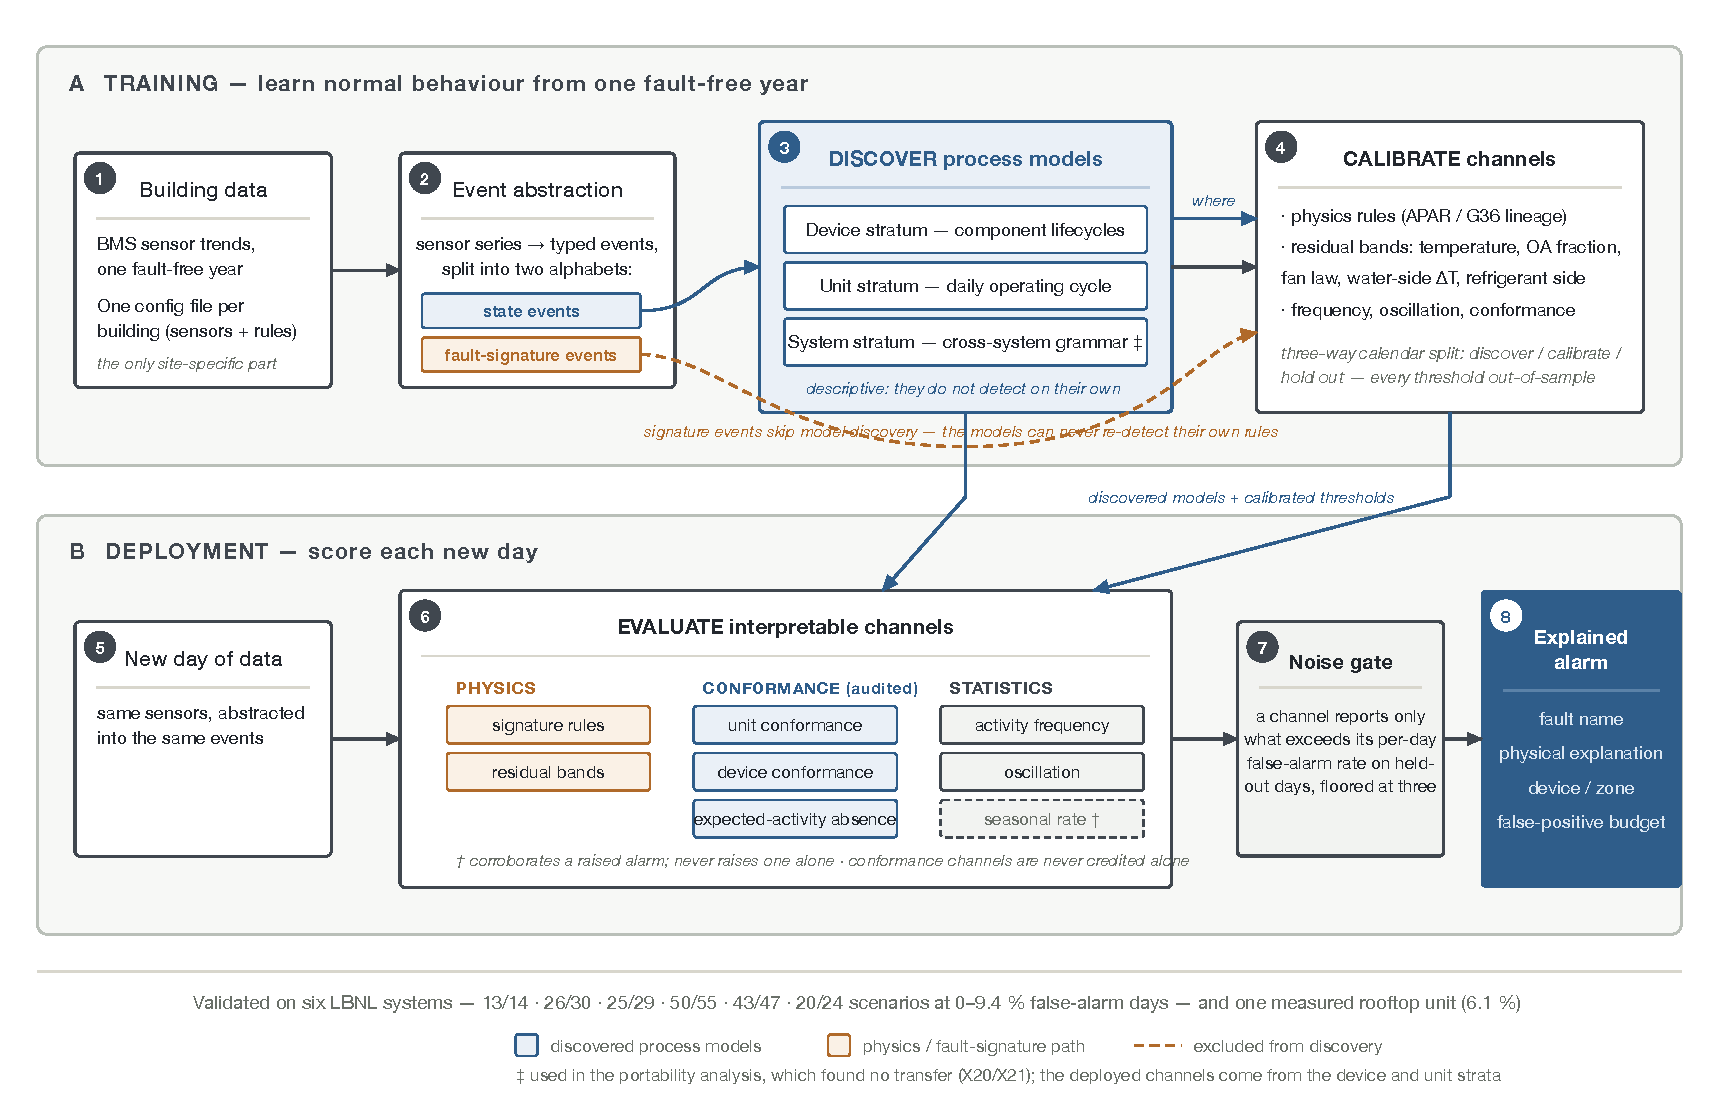
\includegraphics[width=0.92\textwidth]{../figures/strata_framework_v3.pdf}
\caption{The framework as evaluated. Training (top): one fault-free year and one configuration file; events split into state and fault-signature alphabets; process models discovered from state events only; every threshold from a three-way calendar split (discover, calibrate, hold out), so every reported false-alarm rate is out-of-sample. Deployment (bottom): each day is scored by physics, statistical and conformance channels, each reporting only what exceeds its own per-day false-alarm rate; what survives reaches the operator with a name, a physical explanation, the device and the stated budget.}
\label{fig:framework}
\end{figure}

\paragraph{Event abstraction and the alphabet wall.} Continuous streams are converted into a discrete event log by control-sequence rules grounded in Guideline~36 \cite{janssen2021sensoreventlog,vanzelst2021eventabstraction}, then partitioned into two alphabets that are never mixed: \emph{state events}, neutral facts about operation and the only events admitted to discovery, and \emph{fault-signature events}, which encode engineering suspicion and are withheld. The partition exists because of circularity, the process-mining form of data leakage \cite{weytjens2022dataleakage,saydirasulov2026fcu}: a model discovered over an alphabet that names faults will later ``detect'' them by recognising the project's own rules. Against the committed artefact of the pre-partition prototype on the single-duct system, the model channel's apparent recall rises from 1.8\,\% to 5.2\,\% (81 against 238 days) without the partition while every combined-detector number is identical (3{,}152 true positives, 5 false positives): a measured 3.5-point bound on model self-confirmation, and a tested invariant now enforces the wall.

\paragraph{Discovery at three strata.} Petri nets are discovered from the state log with the inductive miner \cite{leemans2013inductiveminer,leemans2014inductiveminerinfrequent} in pm4py \cite{berti2023pm4py} at three granularities: the device stratum models an actuator's lifecycle, the unit stratum the air handler's daily cycle, and a cross-system grammar supports the transfer analysis. Whether a net encodes order at all is what precision metrics address \cite{munozgama2010precision,buijs2012quality,tax2018imprecisions,vandenbroucke2014negativeevents}; we use a direct \emph{reversal probe}, every trace reversed and re-scored. The single-duct net falls from 0.8861 to 0.5526 under reversal; the series fan-powered net scores identically to four decimals (0.9533) and the parallel net shifts by 0.0005 (0.9021 against 0.9026), so neither carries ordering information in its fitness.

\paragraph{Calibrated channels and the noise gate.} Eight channels (Table~\ref{tab:channels}) evaluate each day independently. \emph{Rules} are physics rules of the NIST APAR lineage naming direct contradictions; \emph{residual} bands encode relationships that must hold under known modes (with the cooling coil off, supply minus mixed temperature equals the fan heat rise); \emph{model} and \emph{device conformance} are alignment cost \cite{vanderaalst2012replaying,carmona2018conformancechecking} against the unit and device nets; \emph{absence} flags a scheduled activity that did not occur; \emph{frequency} and \emph{oscillation} are bands on activity counts and reversals; a seasonal \emph{rate} channel corroborates but may not alarm alone. Calibration uses the fault-free year only, at a false-positive quantile of 0.01 against a calendar-stratified holdout of the last eight days of each month; no threshold sees fault data, and every rule needs a positive control, because silence is not competence (a position-based leak rule was structurally deaf on the fan-powered units and was replaced by a waterside flow rule). A channel then reports only what exceeds its own noise floor, tested as a binomial at $p<10^{-3}$ against that channel's false-alarm rate on the held-out days it could evaluate, floored at three, and thresholds are floored at sensor physics: an early result was retracted to at most two detection-days when a 0.5\,$^\circ$F precision floor showed the ``detections'' had cleared a 0.22\,$^\circ$F band by 0.02--0.03\,$^\circ$F. What survives reaches the operator with the implicated device, the evidence and the channel's budget (Figure~\ref{lst:alarm}).

\begin{table}[t]
\centering
\caption{The eight channels as deployed. Every threshold is set from the fault-free year alone; ``alphabet'' names which side of the wall the channel reads. The rate channel is advisory: reported, never counted in the deployed union.}
\label{tab:channels}
\footnotesize\setlength{\tabcolsep}{4pt}
\begin{tabular}{@{}>{\raggedright\arraybackslash}p{1.8cm}>{\raggedright\arraybackslash}p{1.4cm}>{\raggedright\arraybackslash}p{5.2cm}>{\raggedright\arraybackslash}p{4.6cm}>{\raggedright\arraybackslash}p{1.1cm}@{}}
\hline
Channel & Alphabet & A day is flagged when & Threshold source & In union \\
\hline
Rules & signature & a Guideline~36 / APAR-lineage rule fires during operation & fixed bands from the sequence documentation & yes \\
Residual & raw signals & a per-mode physical residual leaves its healthy band & $[\min,\max]$ of training days, widened to the $0.5\,^\circ$F sensor floor & yes \\
Model conf. & state & the day's trace aligns to the unit net below threshold & 1\,\% quantile of per-day fitness, calibration slice & yes \\
Device conf. & state & an actuator's lifecycle trace aligns to its net below threshold & as above, per device net & yes \\
Absence & state & a device active on scheduled training days produces no event on a scheduled day & each device's healthy silence rate & yes \\
Frequency & state & a daily activity count leaves its healthy range & $[\min,\max]$ over training days & yes \\
Oscillation & raw signals & an actuator's daily direction reversals leave their range & $[\min,\max]$ over training days & yes \\
Rate & state & a 30-day active-day rate leaves the month-matched healthy range & training-year windows & advisory \\
\hline
\end{tabular}
\end{table}

\section{Verification as a First-Class Result}
\label{sec:protocol}

Every experiment is pre-registered: the hypothesis and the observation that would refute it are committed before the experiment runs, in the spirit of the hypothesis-testing discipline urged for process mining \cite{pitsch2025hypothesistesting} and of pre-registration templates for predictive modelling \cite{hofman2023preregistration,pawel2022pitfalls}. A falsifier that fires is published as a finding: thirty experiments were run this way (Appendix~\ref{app:ledger}), ten went against the project and all ten are reported (Section~\ref{sec:falsified}). The discipline exists because of a failure mode we observed in ourselves --- one phase report drafted the day of its discovery contained six overclaims, all caught by audit within hours --- and it catches drift: a robustness experiment scored through the importable library detected five dual-duct scenarios the scorecard did not, because the library lacked a repair the scripts had received; a guard now pins the two.

Before any result is computed, a gate battery verifies file integrity, timestamp monotonicity, calendar consistency and rotation, and hashes every derived log so duplicate scenarios cannot pose as independent evidence; a healthy-silence gate confirms each rule set is silent on the fault-free year before it may score anything, and three of the errata of Section~\ref{sec:errata} were found by this battery. Guards run at three levels --- more than a hundred tests on every commit, a regeneration gate that re-derives every committed artefact and diffs it (the single-duct benchmark must reproduce byte-identically), and every validated dataset frozen as a fixture --- and the suite pins three things not ordinarily thought testable: published values, \emph{fired falsifiers} (the sampling-rate finding \emph{is} its four refutations), and \emph{disclosure obligations}, so that a regeneration which drops a published caveat fails the build exactly as a lost feature would. Continuous integration has guarded that a result regenerates \cite{jimenez2017popper}; guarding that a caveat survives is, to our knowledge, new.

Before any number is quoted, it is independently recomputed from raw data by an agent briefed to find it wrong (AI coding agents in this project). The method's value is what it caught: a baseline detecting file provenance rather than faults; one of fourteen single-duct detections that was the dataset's configuration branch, not the fault (14/14 naive, 13/14 adjudicated); a day-level significance test resting on an impossible null, retracted and replaced by the binomial against each channel's own noise; detections below sensor precision; and a completed comparison against commercial practice, voided twice before the execution quoted in Section~\ref{sec:baseline}. None would have been caught by a test suite, because in each case the code did what it was written to do. Simulation flatters, and one measured stream now bounds that: on an LBNL field rooftop unit (182 fault-free days over two summers, 25 points, no schedule point), onboarded by configuration plus one derived fan-on column and two logged silence iterations, the deployed detector's false-alarm rate is 3 of 49 held-out days (6.1\,\%) with every channel inside budget; its one fault case, a 40\,\% refrigerant undercharge, is not seen and is reported as a case, not a rate.

\section{Results}
\label{sec:results}

Evaluation began with three public LBNL datasets \cite{granderson2020lbnlfdddata,granderson2023lbnlfdddata}: a single-duct air handler (SDAHU) and parallel and series fan-powered units (PFPU, SFPU), the latter two never previously benchmarked; a dual-duct air handler (DDAHU) and a fan coil unit (FCU) were onboarded blind afterwards, and a simulated and a measured rooftop unit complete Table~\ref{tab:systems}. Scoring follows day-level, scenario-as-unit conventions \cite{yuill2013fddprotocol,frank2018fddevaluation}; each scenario is a year-long single-fault file, and every false-alarm count is on the 96 held-out fault-free days (the last eight of each month), out-of-sample since the three-way split.

\begin{table}[t]
\centering
\footnotesize
\setlength{\tabcolsep}{3.5pt}
\begin{tabular}{@{}lrrrrrr@{}}
\hline
System (LBNL) & points & rules (state\,/\,sig.) & scored & detected & false alarms & healthy days \\
\hline
SDAHU, single-duct AHU & 26 & 3 / 12 & 14 & 14 (13 adj.) & 1 / 96 & 365 \\
PFPU, parallel fan-powered box & 109 & 13 / 45 & 30 & 26 & 8 / 96 & 365 \\
SFPU, series fan-powered box & 109 & 13 / 49 & 29 & 25 & 9 / 96 & 365 \\
DDAHU, dual-duct AHU & 114 & 15 / 56 & 55 & 50 & 3 / 96 & 365 \\
FCU, fan coil unit & 29 & 7 / 19 & 47 & 43 & 5 / 96 & 365 \\
RTU, simulated rooftop unit & 23$^\dagger$ & 3 / 5 & 24 & 20 & 0 / 28 & 100 \\
RTU, measured rooftop unit (Site 2) & 26$^\dagger$ & 2 / 7 & 1 case & --- & 3 / 49 & 182 \\
\hline
\end{tabular}
\caption{The seven LBNL datasets under the final gate: points mapped after the coverage audit, scenarios scored and detected, and out-of-sample false-alarm days on the held-out fault-free days. The measured unit carries one fault case and is used for its false-alarm rate only. $^\dagger$Includes one derived operating-state column.}
\label{tab:systems}
\end{table}

\paragraph{Detection at a stated budget.} Under the final gate the detector catches 158 of 175 seeded scenarios on the five simulated systems at 26 false-alarm days in 480, the deployed union at 1.0, 8.3, 9.4, 3.1 and 5.2\,\% of held-out days; coil fouling is the dominant miss. The median time to detection is one day on every system and the tail is short: on the single-duct unit 9 of the 13 adjudicated detections come on day 1 and 4 on day 2; on the fan-powered units all 26 and 25 come on day 1. The cry-wolf ratio, wrong alarms as a share of all alarms, is at most 0.13\,\% (0.03, 0.11, 0.12), small partly because fault-scenario days outnumber fault-free days 47--99 to 1. Pooled recall misleads for gated detectors: the coil-bias residual is physics-bound only inside a window (coil off, occupied, sustained 120 minutes) that exists on 137--164 days a year, and within it recall is 164/164, 164/164, 139/139 and 137/137 on the four bias scenarios; the apparent 39--47\,\% ceiling is climate.

\paragraph{The coverage audit.}\label{sec:coverage} The misses remaining after the statistical repair had been read as limits of what the datasets record; a read-only scan found that for six of the fourteen reachable misses the decisive signal was a recorded column no configuration mapped. A pre-registered series (X33a--e) audited every column of every system, mapped every usable one with a physically named reader (a residual, a rule, a gate or an oscillation signal), took every band from the fault-free file, and left the state alphabet untouched, so the process-mining rows had to regenerate byte-identically (Table~\ref{tab:coverage}). Sixteen scenarios were recovered, none lost, five false-alarm days added over 480: airside reheat-coil fouling through the series fan's power per cfm delivered (``same power, less air''), room-temperature biases through the return air falling away from the biased zone, the dual-duct hot-deck biases through the unbiased copies the mixing boxes record, and the fan coil's damper leaks through the outdoor-air fraction. The seventeen remaining misses are coil fouling on every system, whose recorded values sit inside every healthy band on every column; one is visible but uncertifiable from a single healthy year. Two disclosures bound the claim: which columns to read was decided after the scan of the fault files, so the readers were fault-informed though every threshold was blind; and five of the sixteen recoveries sit less than one band width outside the healthy extremes. The series shows these misses were reachable from the recorded columns with blind thresholds, not that a blind onboarding would have reached them; the blind onboardings below are the honest prior for a new building.

\begin{table}[t]
\centering
\small
\begin{tabular}{@{}lrrrr@{}}
\hline
System & columns mapped & detected, before $\to$ after & false alarms, before $\to$ after & lost \\
\hline
SDAHU & 12 $\to$ 26 of 30 & 14 $\to$ 14 / 14 & 1 $\to$ 1 & 0 \\
PFPU & 56 $\to$ 109 of 109 & 22 $\to$ 26 / 30 & 7 $\to$ 8 & 0 \\
SFPU & 56 $\to$ 109 of 109 & 21 $\to$ 25 / 29 & 6 $\to$ 9 & 0 \\
DDAHU & 79 $\to$ 114 of 114 & 45 $\to$ 50 / 55 & 3 $\to$ 3 & 0 \\
FCU & 29 $\to$ 29 of 29 & 40 $\to$ 43 / 47 & 4 $\to$ 5 & 0 \\
\hline
all & 232 $\to$ 387 of 391 & 142 $\to$ 158 / 175 & 21 $\to$ 26 of 480 & 0 \\
\hline
\end{tabular}
\caption{The coverage audit: sixteen scenarios recovered, none lost, five false-alarm days added over 480 held-out days, the model and device rows identical on every system. Totals use the naive single-duct count.}
\label{tab:coverage}
\end{table}

\paragraph{Against a learned baseline.} A principal-component baseline on squared prediction error, audited (it had been detecting file provenance through the columns of erratum E3) and scored on identical universes, detects 61 of the 73 scenarios on the first three systems to STRATA's 64 (13/26/25 against 13/23/25), inside overlapping Wilson intervals ([78.2, 93.4]\,\% against [73.4, 90.3]\,\%); the three discordant scenarios are all STRATA's (an unstable damper and the parallel unit's moderate and severe airside fouling), none the baseline's, and an exact McNemar test on three pairs ($p = 0.25$) is an absence of power, not evidence of superiority. Nine scenarios are missed by both, eight of them reheat-coil fouling. On false alarms the baseline is lower on the terminal units (1/96 against 8/96 and 9/96) and within a day on the air handler (1/79 against 1/96), intervals overlapping throughout; it consumes 108 and 424 raw daily features where STRATA reads physically named relations between mapped columns. What the baseline cannot do is name the implicated device or state the evidence behind a flag.

\begin{figure}[t]
\footnotesize
\begin{verbatim}
STRATA alarm -- series fan-powered unit, 2018-01-01 (day 1 of the fault)
  what      zone primary-air flow not tracking its setpoint   [channel: rules]
  where     terminal unit TU_S, zone S
  evidence  measured 715 CFM against a 200 CFM setpoint -- a 515 CFM excess
            sustained for 720 min while occupied (rule fires at 50 CFM held
            60 min); damper position 0.80, fault-free same-day value 0.32
  budget    rules channel: 0 false-alarm days on the 96-day fault-free
            holdout; threshold set on training days only, holdout out-of-sample
  corrob.   seasonal rate channel agrees (advisory; never alarms alone)
  seeded    zone-S damper stuck at 80% -- location correct, symptom correct,
            detected on day 1 of 365
\end{verbatim}
\caption{A worked alarm, every value read from the committed artefacts and the raw data. Scenario \texttt{SFPU\_VAVDMPRStuck\_80\%}; the alarm names the symptom and its location, not the root cause.}
\label{lst:alarm}
\end{figure}

\paragraph{Localisation and diagnosis.} Every seeded zone fault in the benchmark occurs in the same zone, so attribution is reported as specificity, not discrimination. On the 51 detections on the two fan-powered units in the attribution universe (65 naive detections less the 14 single-duct ones, which have no device stratum), the alarm names the correct terminal unit in 37, names none in 13 and names a wrong unit in none, with one indeterminate; three wrong units were available in every case, so the zero is falsifiable. A pre-registered component test (X34) over all 158 detections found the carrying rule naming the seeded component exactly in 109 (69\,\%), the right subsystem in 22 more (14\,\%), the wrong subsystem in 20 (12.7\,\%) and no component in 7; the bar for a component-level claim (wrong subsystem $\le 10\,\%$) was missed, so the claim is subsystem-level. Fourteen of the twenty wrong cases are on the single-zone fan coil unit and name the component that responds to the fault, the first place a technician would look. A pre-registered diagnosis layer (X37) of three fault-agnostic ingredients --- the sign of every significant residual, a consensus rule over redundant copies of one quantity, and a leave-one-out nearest-pattern vote for the fault family --- resolved the five dual-duct damper cases the carrying rule had scored wrong (one mixing-box copy moves alone) and called 14 of 16 deck sensor biases at the deck, lifting exact attribution to 112 of 158 (71\,\%) and exact-or-subsystem to 85\,\%, with the wrong-subsystem rate at 10.1\,\%. It missed its own bars --- the family is named from the signed pattern alone in 85 of 114 resolved detections (74.6\,\%, bar 80) with 44 unresolved (27.8\,\%, bar 15), because a stuck damper and a biased airflow sensor, a restricted filter and a fouled coil, a leaking and a stuck valve are pairs the recorded quantities cannot separate by sign --- so it is not adopted. What the framework can honestly say is what it measured: zone right and never wrong, subsystem right in 85\,\%, exact component in 71\,\%.

\paragraph{Onboarding blind.} The claim that a building is a configuration directory was tested on two system types the project had never seen, under pre-registrations written after the documentation and before any data file was opened. The dual-duct unit (55 faults in 15 families, two new) took 79 mappings, 15 state and 26 signature rules and one healthy-silence iteration (ten days on which the cold-deck fan saturates, removed by a physical gate rather than a looser threshold) and scored 45 of 55 at 3 false-alarm days in 96 with no code change (50 after the coverage audit). The fan coil unit (47 scored faults in 17 families, four new) took 29 mappings and 7 state and 16 signature rules; its first run scored 47 of 47 at 28 false-alarm days and fired two falsifiers, because two scoring scripts written for the fan-powered units treated an event-less setback day as a scheduled model violation, and a pre-registered repair restored 41 of 47 at 4 false-alarm days with the four earlier scorecards regenerating byte-identically (43 after the coverage audit). The second system type had been onboarded in about 1.5 hours, 45 mappings and 35 rules; the third was derived from it in minutes.

\paragraph{Field conditions and calibration.} On the shipped configurations of all five systems after the coverage audit (X35), field sensor error on temperatures, flows and positions, change-of-value logging with stale repeats and gaps, and schedule shifts with holidays, each and all together, applied to the fault-free year and every fault file and re-fitted, kept the budget in every cell (worst 7 of 96, the parallel unit under the schedule shift; no system more than two above its clean count), cost at most one detection per system and condition, gained nothing, and reproduced the scorecard on the clean arm; of the five edge recoveries one was lost under noise, where the pre-registration predicted at least two. A pre-registered alternative calibration (X36), bands at the 2nd and 98th percentiles of the training days instead of the extremes, about ten per cent narrower, gained no scenario and lost none, kept all five edge recoveries, and added thirteen residual false-alarm days over 480, four each on the fan-powered units; its budget falsifier fired and the deployed $[\min,\max]$ calibration is unchanged. Earlier tests: under i.i.d. jitter at sensor precision the counts are unchanged and under a mirrored holdout they move by at most one, while the membership of the marginal scenarios shifts; and a single score-carrying contaminated training day collapses the two negative coil-bias rungs from 164 of 164 detections to none, the mild contamination source visible on 100\,\% of its days (5/5, 13/13, 27/27) and the dangerous one on none of its 27.

\subsection{What process mining carries, and what it does not}
\label{sec:pm}

The stratified structure is what makes the alarm of Figure~\ref{lst:alarm} possible: the device stratum is why an alarm names a terminal unit, and the single-duct system, which has none, names no device by construction. The event log carries detections of its own: the frequency channel measures count deviations two-sidedly and was significant on 12 of the 61 scenarios the scorecard then detected on the first three systems; the oscillation channel stands alone on the unstable-damper scenario, 349 detections against at most two from any hand-written rule; seven detections across the five systems are carried by the frequency or oscillation channel alone, instability faults and one fan restriction that no rule names; and on the dual-duct unit a day-one alarm belongs to the absence channel. A matched-rule control isolates what discovery contributed at design time: for each channel a hand-written equivalent was authored, and two reproduce their channel exactly (141 against 141 detections on the series unit, 206 against 206 on the parallel unit) --- the discovered models surfaced invariants an expert then wrote as rules.

Conformance checking of the discovered nets is a different matter, and the result is measured. Reading the significance-gated channel credited with each detection from the committed scorecards, no scenario on any of the six systems is detected only by the two conformance channels: they are credited with none of the single-duct or parallel-unit detections and appear in 7 of 25 on the series unit, never alone. Removing them changes no scorecard and lowers the series unit's false-alarm rate from 9/96 to 4/96 and the parallel unit's from 8/96 to 6/96; over 199 scenarios the one-sided 95\,\% upper bound on the sole-detection rate is 1.5\,\%. The log explains why: under waterside reheat-coil fouling the state-event log is identical to healthy to the minute, eight of the twelve scenarios then missed have a log indistinguishable from healthy at a 5\,\% tolerance, so no method that reads that log can detect them, and under a 50\,\% reheat-valve leak the log changes in timing and counts with its order unchanged, which control-flow conformance cannot see by construction. Three pre-registered extensions followed. A time-infused state model (X12) is significant on 11 of 73 scenarios and on none the deployed channels miss, at five extra false-alarm days per fan-powered unit. Healthy-derived band states for every actuator and flow (X14) enrich the alphabet by 6, 40 and 36 events; the single-duct model channel then fires on all 14 scenarios instead of none and one miss, moderate airside fouling of a series-unit reheat coil, becomes significant through a dose-monotone zone-damper signature, at 7, 18 and 21 false-alarm days in 96, over budget, so that falsifier fired. The enriched frequency channel alone (X15) keeps that one gain inside the budget under two splits, a candidate addition rather than an adopted one, and does not replicate on the dual-duct unit (X18).

A pre-registered positive control settled whether the channel can see order at all: injected violations (reversal, adjacent swaps, deletions, a deleted start, a duplicated block) scored on each system's fault-free holdout with the deployed net and gate. The channel is three instruments. On the fan coil and dual-duct units a reversed day is flagged on 55 of 72 and 59 of 83 holdout days (AUC 0.99): the channel sees order and those units' faults do not change it. On the single-duct unit a reversed day is separable on average (AUC 0.91) but the healthy holdout contains days that fit worse than a reversed one, so no in-budget threshold sees order. On the fan-powered units fitness does not move under any perturbation (AUC 0.36--0.51): blind by net structure. A grid of seven process-mining instruments (X30), from the heuristics miner and token replay to the log skeleton, Declare constraints and the temporal profile, thresholded and gated as every channel is, detects none of the 33 scenarios the detector then missed at realised false-alarm rates of 0 to 9.7\,\%: the null is a property of the state-event log, not of the miner or the measure. Sixteen of those 33 were later recovered by the coverage audit, through columns no process model was ever given.

\subsection{Against current practice: the falsifier fired}
\label{sec:baseline}

The comparison practitioners care about is against the rule-based detection deployed in commercial automation systems \cite{granderson2017fddtoolsurvey}. A third-party open-source implementation of the Guideline~36 fault conditions, open-fdd 4.4.1 \cite{openfdd2025}, was imported at its installed defaults, air handlers graded with the standard's fifteen conditions and terminal units with the library's terminal-unit rules per zone, on the identical examination; the pre-registered refutation condition was that the battery matching STRATA's count at equal or lower false alarms on any system would abandon the improvement claim there. Two executions were voided first, the second after two independent audits found six adapter defects and a pooled gate that is a tautology once the union flags every healthy day; an amendment recorded them before the third execution, which is quoted (Table~\ref{tab:g36}).

\begin{table}[t]
\centering
\small
\setlength{\tabcolsep}{5pt}
\begin{tabular}{@{}lccc@{}}
\hline
 & SDAHU (14) & PFPU (30) & SFPU (29) \\
\hline
Battery, pooled gate (as first registered) & 1 @ 49 & 0 @ 96 & 0 @ 96 \\
Battery, per rule against its own holdout rate & 12 & 30$^\dagger$ & 29$^\dagger$ \\
Battery, rules silent on the healthy year, held to 3/365 & 12 @ 1 & 8 @ 0 & 9 @ 0 \\
STRATA, deployed & 13 @ 1 & 26 @ 8 & 25 @ 9 \\
\hline
\end{tabular}
\caption{The repaired Guideline~36 battery against STRATA: scenarios detected @ false-alarm days in 96. $^\dagger$Not detection: three air-handler conditions flag the identical day sets on the fault-free file and every fault file and pass only because each rule's holdout rate sits below its full-year rate; excluding the self-detecting rules post hoc gives 15 of 30 and 17 of 29. STRATA's single-duct count is 13 by the branch adjudication of erratum E5, which the battery's count does not apply.}
\label{tab:g36}
\end{table}

Held to STRATA's own treatment of its signature rules --- keep the rules silent on the fault-free year and hold them to the same 3/365 null --- the battery detects 12 of 14 on the single-duct air handler at one false-alarm day against STRATA's 13 at one (its two misses are the 10 and 25\,\% stuck dampers, seen only by a condition that is not silent), and 8 of 30 and 9 of 29 on the terminal units at no false-alarm day against STRATA's 26 and 25 at eight and nine. The falsifier fired on every system --- on the air handler because equal false alarms is a match, on the terminal units because none is fewer --- so the pre-registered improvement claim cannot be made. What the artefact supports is narrower: on the air handler a correctly wired Guideline~36 battery, silenced on the fault-free year, is within one detection and one false-alarm day of STRATA; on the terminal units STRATA detects three times as many seeded faults and pays eight or nine false-alarm days in 96 for them, and the difference is coverage, the per-zone residual readers of the coverage audit, not the gate. Four caveats travel with the numbers: the battery's rule selection is judged on the whole fault-free year including the holdout, so its one false-alarm day is a post-selection count where STRATA's is out of sample; the outdoor-air-bias file is adjudicated away on STRATA's side only (removing it from both gives 11 of 13 against 13 of 13); the parameters are open-fdd's installed defaults, tighter on every condition that fired than the Guideline~36 values the library cites; and the terminal rules carry fixed comfort bands that do not read the building's setpoint columns.

\section{What the Protocol Refuted or Withdrew}
\label{sec:falsified}

Ten results went against the project; each is reported with what survived. (1)~\emph{Discovered models do not out-detect hand-written rules.} On the series-unit scenario where the unit net was strongest (zone-damper faults erase the daily heating rhythm), a one-line matched rule --- occupied workday and heating never active, zero false alarms on 365 healthy days --- covered 192 days against the model channel's 135 (178 in the current artefact); the falsifier fired and the rule is a permanent ablation arm. (2)~\emph{Behavioural structure does not transfer zero-shot.} Fan-powered logs outscore their shuffled controls on the single-duct net by 0.15 and 0.18 in fitness, but the detection hypothesis yielded zero to one gated detection per rotation; portability is claimed at configuration level only. (3)~\emph{The models' detections were count deviations in disguise}, surfacing through alignment cost; once the frequency channel measured them directly the conformance channels had nothing uniquely theirs (Section~\ref{sec:pm}). (4)~\emph{14 of 14 became 13 of 14} when an audit found the single-duct fault-free file simulated on a different configuration branch than every fault file (erratum E5): under a branch-corrected band that scenario's only channel produced zero flags on 148 window days. (5)~\emph{A day-level significance test was retracted}: its discordant cell was zero by construction, and thirteen parallel-unit rows lost their stars. (6)~\emph{Healthy silence does not survive resampling}: configurations tuned at one-minute sampling gain 28 to 64 spurious healthy signature-days at fifteen minutes; four falsifiers fired, and the silence gate is re-run at the deployment sampling rate. (7)~\emph{A pre-registered transfer test never had power.} Whether model support predicts where a transplanted rule holds was tested with quantity, predictions and falsifiers sealed, but the model quantity is constant within a building (0.000, 0.455, 0.978), so nine cells were three buildings pseudo-replicated and the valid null has minimum $p = 1/3! = 0.167$ against a criterion of 0.05; three dated amendments record it, the reported $p = 0.20$ is not a measurement, and no inference is drawn. (8)~\emph{A fault-informed coil-effectiveness residual} was significant on one of twelve fouling scenarios, already detected; its falsifier fired. The positive control is LBNL's simulated rooftop unit, the one dataset recording the refrigerant side, where the unchanged detector catches every condenser- and evaporator-fouling severity down to 10\,\% (10 of 10, monotone) at 0 false-alarm days in 28. (9)~\emph{Richer vocabulary buys detections at false alarms the budget forbids} (X14, Section~\ref{sec:pm}). (10)~\emph{The powered transfer re-run passed for the wrong reason.} With four scorable buildings the pre-registered identity test gives $\rho = -1$, exact $p = 1/24 = 0.042$, and the artefact records the pass as licensed; the paper declines it because a discovery-free control, the raw heating-day fraction, orders the buildings identically, and the non-circular variant, a net fitted on one building reading another's year (X21), orders them no better ($\rho = -0.6$).

\section{Defects in the Benchmark Datasets}
\label{sec:errata}

Auditing the evaluation produced eight defects in the LBNL benchmark datasets (Table~\ref{tab:errata}), each with machine-verifiable evidence and a reproducing command in the repository's ERRATA.md; the creators' own account of the models' fidelity limits \cite{casillas2024ahufaultmodels} is the closest prior. The most consequential for other researchers is E3: a single threshold on either static-pressure column, chosen from the fault-free file alone, classifies all 365 fault-free days and all 7{,}150 fault days correctly, so any model given those columns identifies provenance perfectly without reference to any fault. Published results on this dataset that used the full column set should be read with that in mind.

\begin{table}[t]
\centering
\scriptsize
\setlength{\tabcolsep}{4pt}
\renewcommand{\arraystretch}{1.05}
\begin{tabular}{@{}>{\raggedright\arraybackslash}p{0.5cm}>{\raggedright\arraybackslash}p{1.3cm}>{\raggedright\arraybackslash}p{7.2cm}>{\raggedright\arraybackslash}p{6.3cm}@{}}
\hline
ID & System & Defect & Consequence \\
\hline
E1 & SDAHU & \texttt{oa\_bias}: one run shipped four times under different severity labels; the labelled sensor-side bias never appears in the logged column. & Four labels index one run; the mechanism is not asserted. \\
E2 & SDAHU & \texttt{coi\_leakage}: one run shipped four times under different severity labels. & Four labels index one run; the family is scored once. \\
E3 & SDAHU & A constant of about 401.86 added to \texttt{SA\_SP} in the fault-free file and subtracted from \texttt{SA\_SPSPT} in every fault file, ranges disjoint. & Either column separates healthy from fault by provenance; both excluded from all baselines. \\
E4 & SFPU & \texttt{SensorBias\_RMTEMP\_-2C}: calendar rotated relative to its siblings. & Excluded; the SFPU universe is 29. \\
E5 & SDAHU & The healthy file was simulated on a different configuration branch than every fault file (occupied damper floor 0.0 against 0.1, different schedules). & One detection was provenance; 14/14 naive, 13/14 adjudicated. \\
E6 & FCU & Two minor airside-fouling files (cooling, heating) are byte-identical. & One label is wrong; scored once, the FCU universe is 47. \\
E7 & PFPU, SFPU & Documentation places every seeded fault in the west zone; in every file only the south zone's columns move (57 of 60; three indeterminate). & Localisation scored against the documented zone would mark every correct alarm wrong; ground truth taken from the data. \\
E8 & DDAHU & Static-pressure bias files: the deck column is unchanged and the box statics shift by one tenth of the labelled bias. & Severity ladders built from these labels are off by ten; detections unaffected. \\
\hline
\end{tabular}
\caption{Eight machine-verified defects in the LBNL benchmark datasets.}
\label{tab:errata}
\end{table}

\section{Limitations}
\label{sec:limitations}

All detection results come from simulation, and simulation flatters; the field-condition injections and the one measured stream narrow the gap without closing it. The measured rooftop unit supports a false-alarm rate and one unseen fault case, and until deployment on an operating building is complete the framework is validated in the laboratory; the contamination result bears on that gap directly, because a real building's baseline year is not fault-free by construction.

Two reporting decisions are disclosed. The deployed rates treat the seasonal rate channel as corroborating evidence that may not alarm alone; the naive union of all eight channels false-alarms on 15.6\,\% of held-out days on the single-duct system, nearly all of it that channel, the demotion was adopted after those figures were known and costs no detection, and readers comparing against an undemoted union should use 15.6\,\%. Second, until the three-way split the conformance channels' holdout rows were calibration targets rather than measurements; the split measured that debt (the fan-powered budgets moved from 5.2 and 4.2 to 7.3 and 6.2\,\%), and making the residual channel's null a per-day rate then removed seven residual-only detections, a loss that fired a pre-registered falsifier and is reported as a detector change.

The noise-floor gate applies no correction across channels and scenarios: on the order of 1{,}600 binomial tests at $\alpha = 10^{-3}$ give a family-wise error near 0.8 under independence, about 1.6 false cells across the study, and per-day observations within a scenario are autocorrelated. All counts are single-run figures on one simulated year per system; gradually developing faults are detected slowly, the expected cost of calibrating below a noise floor; the component-level attribution claim and the diagnosis layer both missed their pre-registered bars, and the alarm names a symptom and a location, not a root cause. The hybrid extension is deferred deliberately, because the test worth running is whether it detects more at an equal budget while still naming the device. Six simulated systems across five equipment classes demonstrate configuration-level portability, not generality across commercial HVAC; a 2026 collection of eight further labelled AHU datasets \cite{ghalamsiah2026ahudatasets} is the obvious next target.

\section{Conclusion}

STRATA does what its intent asks on the benchmarks it was tested on: from one fault-free year and one configuration file it detects 158 of 175 seeded faults on five public systems at 26 false-alarm days in 480, most on the first day, names the terminal unit correctly and never wrongly, the subsystem in 85\,\% of detections and the exact component in 71\,\%, and issues each alarm with the evidence behind it and the channel's own false-alarm budget --- properties a scalar anomaly score of equal detecting power cannot supply. Process mining is what makes that structure possible, and its contribution is now measured rather than assumed: the strata name the device, the event abstraction from the control sequence is the vocabulary, and the absence, frequency and oscillation channels over the log carry detections no rule names; conformance checking of the discovered nets alone detects no fault the other channels miss. Process mining helps to get detection; it is not detecting on its own. The protocol --- thirty pre-registered experiments, ten adverse outcomes honoured, eight benchmark defects documented with reproducible evidence --- is offered as a contribution in its own right: in a subfield where independent verification is rare, a result that has survived a genuine attempt at refutation is worth more than a larger number that has not.

\section*{Acknowledgements}
The author thanks Dr.\ Anthony Aighobahi and Dr.\ Mridula Sharma for supervision throughout this project. AI coding assistants were used for implementation, analysis scripting and adversarial auditing of results; all experimental designs, pre-registrations and claims were reviewed and approved by the author.

\bibliographystyle{plain}
\bibliography{../references}

\appendix
\section{Every pre-registered experiment}
\label{app:ledger}

Tables~\ref{tab:ledger} and \ref{tab:ledger-b} list every pre-registered experiment in the order it was run, with its prediction, outcome and what fired. Each row resolves to a ledger under \texttt{outputs/} or, where noted in the repository's research log, to the phase report; amendments are folded into the row they amend.

\begin{table}[p]
\centering
\footnotesize
\setlength{\tabcolsep}{3pt}
\renewcommand{\arraystretch}{1.05}
\begin{tabular}{@{}>{\raggedright\arraybackslash}p{1.1cm}>{\raggedright\arraybackslash}p{4.6cm}>{\raggedright\arraybackslash}p{3.3cm}>{\raggedright\arraybackslash}p{4.3cm}>{\raggedright\arraybackslash}p{2.2cm}@{}}
\hline
ID & Experiment & Prediction & Outcome & Falsifier \\
\hline
--- & Do discovered unit models out-detect a hand-written rule? & Model channel covers more fault days than any matched rule & Matched rule 192 days against the model channel's 135 (178 now) at 0 of 365 healthy false alarms & Fired \\
--- & Does behavioural structure transfer zero-shot? & Source-fitted bands detect on the target & 0 of 14 single-duct scenarios under the confidence-bound gate & Fired \\
--- & Does model support predict where a transplanted rule holds? (three amendments) & $\rho < 0$, permutation $p < 0.05$ over nine cells & $\rho = -0.69$, $p = 0.200$; valid null over three buildings has minimum $p = 0.167$ & F1, F2 fired, then voided; no power \\
X5 & Are severity ladders monotone in dose? & No ladder significantly anti-monotone & Series-unit fouling $\rho = +0.87$; none anti-monotone & None \\
X7 & Does healthy silence survive 15-minute resampling? & Signature days and residual coverage preserved & Healthy years gain 28, 64 and 64 signature days; one residual's coverage falls 31 to 1 & F-X7.a (three systems), F-X7.b \\
X8 & Does training contamination break extreme-value calibration? & Breakdown at small contamination; mild sources visible & One contaminated day collapses both negative coil-bias rungs, 164 of 164 to 0 & None \\
X9/X10 & Robust to sensor jitter and to the holdout split? & Detections change by at most 3; false alarms under 10\,\% & Unchanged at $1\times$ jitter, within one on the mirrored split; 0--4 false alarms of 96 & None \\
X11 & Is the single-duct OA-bias detection the fault or the branch? & Five estimators agree; the branch offset explains the flags & Offset $+1.06\,^\circ$F; 0 flags on 148 window days; 14/14 becomes 13/14 & F-X11.d (run 1); leg re-specified \\
X12 & Does the time perspective recover missed scenarios? & Duration channel newly detects missed scenarios & 11 significant, 0 newly detected & None; P3 failed \\
X13 & Does a coil-effectiveness residual separate reheat fouling? & At least 6 of 9 fouling scenarios significant & 1 of 12, already detected elsewhere & F-X13.b \\
X14 & Was the model starved of vocabulary? & One new detection inside the budget & One new; model channel fires on 14 scenarios; 7, 18, 21 false alarms of 96 & F-X14.a (budget) \\
X15 & Does the enriched gain survive frequency-only scoring under two splits? & Significant under both, inside budget & Same one scenario under both; 41 significant against 12 deployed & None \\
X17 & Dual-duct AHU onboarded by configuration alone? & Config-only, gates clean, $\ge 60\,\%$ detected & 45 of 55 at 3 false alarms of 96; one silence iteration & None; P6 failed (5 fouling, not $\le 4$) \\
X18 & Does the enriched-frequency gain replicate on the dual-duct unit? & A missed fouling scenario becomes significant & 0 newly significant; 22 against 8 on already-detected & F-X18.b \\
X19 r1 & Fan coil unit onboarded by configuration alone? & Gates clean, $\le 10$ false alarms, no conformance-only scenario & 47 of 47 at 28 false alarms; 6 conformance-only & F-X19.b, F-X19.d \\
X19 A1 & Does the amended onboarding hold? & Budget restored, no conformance-only detection & 41 of 47 at 4 false alarms; 0 conformance-only & None \\
X20 & Is model support the log's own heating-day count across four buildings? & Identity holds; $\rho < 0$ at $p < 0.05$ & $\rho = -1$, $p = 1/24 = 0.042$; identity misses by 44 days on the fan coil unit & F-X20.a, F-X20.b \\
X21 & Can a net's reading of a foreign year escape being that log's count? & Bound holds, tautology persists, ordering matches & Tautology fails on 6 of 12 pairs; foreign predictor $\rho = -0.6$ & F-X21.a; P3 failed \\
X22 & Does the conformance channel fire on injected order violations? & Reversal significant on the single-duct unit & Significant on 2 of 5 systems; single-duct hit rate 0 at zero false alarms & None; P1--P4 failed \\
\hline
\end{tabular}
\caption{Every pre-registered experiment, its prediction, its outcome and what fired (part 1 of 2).}
\label{tab:ledger}
\end{table}

\begin{table}[p]
\centering
\footnotesize
\setlength{\tabcolsep}{3pt}
\renewcommand{\arraystretch}{1.05}
\begin{tabular}{@{}>{\raggedright\arraybackslash}p{1.1cm}>{\raggedright\arraybackslash}p{4.6cm}>{\raggedright\arraybackslash}p{3.3cm}>{\raggedright\arraybackslash}p{4.3cm}>{\raggedright\arraybackslash}p{2.2cm}@{}}
\hline
ID & Experiment & Prediction & Outcome & Falsifier \\
\hline
X24 & Does an outdoor-air-fraction residual add detections? & 20\,\% damper leak detected, budget held & Fan coil 41 to 42 of 47 at 4 false alarms & None \\
X25 1--2 & Are the conformance thresholds calibrated out of sample? & Rows out of sample, budget $\le 10$, $\le 3$ verdict flips & Held at 0 flips; in-sample rows had understated false alarms by 3 and 4 days & None \\
X25 3 & Does a max(fp,3)/n floor keep verdicts? & Counts within 2, $\le 3$ flips & 2 flips; one gained, one lost & None \\
X25 4 & Does a per-day residual null keep the detections? & Each count within 2 & Series unit loses 3, 8 verdicts flip & F-X25.c \\
X26 (+A1) & Does the budget hold on a real building? & $\le 3$ silence iterations, false alarms under 10\,\%, fault case flagged & 6.1\,\% false-alarm days, every channel in budget; the 40\,\% undercharge not flagged & None; case predictions failed \\
X27 & Does a fan-law virtual static recover static-pressure biases? & $\ge 7$ of 8 detected & 6 of 8; budget held & F-X27.b \\
X28 & Does a water-side coil UA channel see the simulated fouling? & $\ge 3$ dual-duct and 2 fan coil fouling gained & 0 gained; run 1 also broke the fan coil budget & F-X28.b; run 1 F-X28.a \\
X29 & Is fouling visible when the refrigerant side is recorded? & $\ge 3$ of 5 condenser and evaporator severities, monotone & All 10 detected, monotone, 0 false alarms of 28 & None \\
X30 & Does any other process-mining instrument see the deployed misses? & No cell detects a miss within 3 false alarms & 0 detections over 33 cells; worst cell 7 of 72 & F-X30.b (two cells not evaluated) \\
X31 (+A1) & Field noise, change-of-value logging, schedule shifts? & Budget held; schedule arm within $\pm 1$ & Budgets held; dual-duct schedule arm 48 against 45 & None; P3 and A1 failed \\
X33a--e & Does mapping every recorded column recover the misses? & No loss; budget $\le$ clean $+ 3$ & 142 $\to$ 158 of 175, none lost, 21 $\to$ 26 of 480 & None; three predictions failed upward, one downward \\
X34 & Does the carrying rule name the seeded component? & Exact $\ge 60$; exact or subsystem $\ge 85$; wrong $\le 10\,\%$ & Exact 69\,\%, subsystem 14\,\%, wrong 12.7\,\%, unnamed 7 & F-X34.a; claim withdrawn \\
X35 & Field conditions on the post-coverage configurations? & Budget $\le$ clean $+ 3$; $\ge 2$ edge recoveries lost under noise & Worst 7 of 96; at most one detection lost per cell; one edge recovery lost & None; P3 failed \\
X36 & Do percentile bands keep the edge recoveries in budget? & False alarms rise $\le 3$; $\ge 2$ new detections & Nothing gained or lost; $+4$ on both fan-powered units & F-X36.a \\
X37 (3 runs) & Do signed patterns and consensus diagnose family and component? & Family $\ge 80\,\%$, unresolved $\le 15\,\%$; wrong $< 10\,\%$ & Family 74.6\,\%, unresolved 27.8\,\%; wrong 10.1\,\%; dual-duct damper cases resolved & F-X37.a, F-X37.b \\
X38 (+A1) & Does the repaired Guideline~36 battery match STRATA under the same gate? & STRATA at least as many at lower false alarms & Silent-rule battery 12 of 14 @ 1 vs 13 @ 1; 8 of 30 and 9 of 29 @ 0 vs 26 and 25 @ 8 and 9 & F-X38.a (G2, G3, S) \\
\hline
\end{tabular}
\caption{Every pre-registered experiment, its prediction, its outcome and what fired (part 2 of 2).}
\label{tab:ledger-b}
\end{table}

\end{document}
